% -*- mode: latex; -*- mustache tags:  
\documentclass[10pt,twoside,english]{_support/latex/sbabook/sbabook}
\let\wholebook=\relax

\usepackage{import}
\subimport{_support/latex/}{common.tex}

%=================================================================
% Debug packages for page layout and overfull lines
% Remove the showtrims document option before printing
\ifshowtrims
  \usepackage{showframe}
  \usepackage[color=magenta,width=5mm]{_support/latex/overcolored}
\fi


% =================================================================
\title{Learning Object-Oriented Programming, Design and TDD with Pharo}
\author{Stéphane Ducasse}
\series{The Pharo TextBook Collection}

\hypersetup{
  pdftitle = {Learning Object-Oriented Programming, Design and TDD with Pharo},
  pdfauthor = {Stéphane Ducasse},
  pdfkeywords = {Introduction, programming, design, testing, Pharo, Smalltalk}
}


% =================================================================
\begin{document}

% Title page and colophon on verso
\maketitle
\pagestyle{titlingpage}
\thispagestyle{titlingpage} % \pagestyle does not work on the first one…

\cleartoverso
{\small

  Copyright 2017 by Stéphane Ducasse.

  The contents of this book are protected under the Creative Commons
  Attribution-ShareAlike 3.0 Unported license.

  You are \textbf{free}:
  \begin{itemize}
  \item to \textbf{Share}: to copy, distribute and transmit the work,
  \item to \textbf{Remix}: to adapt the work,
  \end{itemize}

  Under the following conditions:
  \begin{description}
  \item[Attribution.] You must attribute the work in the manner specified by the
    author or licensor (but not in any way that suggests that they endorse you
    or your use of the work).
  \item[Share Alike.] If you alter, transform, or build upon this work, you may
    distribute the resulting work only under the same, similar or a compatible
    license.
  \end{description}

  For any reuse or distribution, you must make clear to others the
  license terms of this work. The best way to do this is with a link to
  this web page: \\
  \url{http://creativecommons.org/licenses/by-sa/3.0/}

  Any of the above conditions can be waived if you get permission from
  the copyright holder. Nothing in this license impairs or restricts the
  author's moral rights.

  \begin{center}
    
\includegraphics[width=0.2\textwidth]{_support/latex/sbabook/CreativeCommons-BY-SA.pdf}
  \end{center}

  Your fair dealing and other rights are in no way affected by the
  above. This is a human-readable summary of the Legal Code (the full
  license): \\
  \url{http://creativecommons.org/licenses/by-sa/3.0/legalcode}

  \vfill

  % Publication info would go here (publisher, ISBN, cover design…)
  Layout and typography based on the \textcode{sbabook} \LaTeX{} class by Damien
  Pollet.
}


\frontmatter
\pagestyle{plain}

\tableofcontents*
\clearpage\listoffigures

\mainmatter

\chapter{Pharo's syntax overview}\label{cha:syntax}
Pharo syntax is minimal: The complete syntax fits in one postcard.
Pharo syntax is based on a couple of constructs such as \textit{variable definition}, ' \textit{assignment}, \textit{return}, \textit{sequence}, and two main construct used systematically: \textit{messages} and \textit{blocks}.  This chapter provides some basic introduction to the key points. There will be not much more but the reader willing to get a deep and precise presentation of syntax should read the corresponding chapters in Pharo By Example available at \url{http://books.pharobyexample.org}
\section{Minimal}
Pharo's syntax is minimal. Essentially there is syntax only for sending messages
(i.e., expressions). Expressions are built up from a very small number of
primitive elements (message sends, assignments, closures, returns...). There are
only a couple a special variables, and there is no syntax for control structures or declaring new
classes. Instead, nearly everything is achieved by sending messages to objects.
For instance, instead of an if-then-else control structure, conditionals are
expressed as messages (such as \textcode{ifTrue:}) sent to Boolean objects. New
(sub-)classes are created by sending a message to their superclass.

Although Pharo's message syntax is simple, it is unconventional. This chapter offers some guidance to help you get
acclimatized to this special syntax for sending messages. If you already feel
comfortable with the syntax, you may choose to skip this chapter, or come back
to it later.
\section{Literal objects}
In Pharo, most objects are created by sending the message \textcode{new} to a class. There are also some objects that are directly created by the compiler. 
\subsection{Comments}
Comments are delimited by double quotes \textcode{\symbol{34}}. 

\begin{displaycode}{plain}
"Hello"
\end{displaycode}
\subsection{Characters, Strings and Symbols}
Characters short form creation is following the pattern dollar sign followed by the letter.  The expression \textcode{\$A} is the character A.

\begin{displaycode}{plain}
$A
>>> $A
\end{displaycode}

Strings are delimited by single quotes \textcode{'}.

\begin{displaycode}{plain}
'Hello'
>>> 'Hello'
\end{displaycode}

Strings are sequence of characters.

\begin{displaycode}{plain}
'Hello' first
>>> $A
\end{displaycode}

We can concatenate strings using the message \textcode{,}.

\begin{displaycode}{plain}
'Hello ', 'Pharoers'
>>> 'Hello Pharoers'
\end{displaycode}

Symbols are unique strings. They start with \textcode{\#}.

\begin{displaycode}{plain}
#'Hello Pharoers'
>>> #'Hello Pharoers'
\end{displaycode}
\subsection{Booleans}
There are two Booleans \textcode{true} and \textcode{false}. 

\begin{displaycode}{plain}
true not
>>> false
\end{displaycode}
\subsection{Arrays}
Arrays can be created as any other objects by sending the message \textcode{new} to the class \textcode{Array}.
In addition, Pharo supports two other ways: \textcode{\#( )} and \textcode{\{ . \}}. 

The expression \textcode{\#(1 + 2 3)} creates an array with four objects: 1, \textcode{\#+}, 2, and 3. 

\begin{displaycode}{plain}
#(1 + 2 3)
>>> #(1 + 2 3)
\end{displaycode}

The expression \textcode{\{1 + 2\}} creates an array with one object resulting from the expression \textcode{1 + 2}.

\begin{displaycode}{plain}
{ 1 + 2}
>>> #(3)
\end{displaycode}

The expression \textcode{\{1 + 2 . 3 + 4\}} creates an array with two objects resulting from the execution of expressions separated by period.

\begin{displaycode}{plain}
{ 1 + 2 . 3 + 4}
>>> #(3 7)
\end{displaycode}
\section{Key expressions}
In Pharo, except for a few constructs (\textcode{:= \string^ . ; \# () \{\} {[} : \textbar{} {]}} ), everything else is a message send.
There is no operators or control flow constructs,  just messages sent to objects. Therefore you can 
define a message named \textcode{+} in your class. 
\subsection{Variable definition and assignment}
The expression \textcode{\textbar{} sum \textbar{}} declares a local variable. The expression \textcode{ sum := 0} changes the value of the variable \textcode{sum} to 0. The assignment construct is \textcode{:=}.

\begin{displaycode}{plain}
| sum |
sum := 0
\end{displaycode}
\subsection{Special variables}
There are several special variables:

\begin{itemize}
\item \textcode{nil} is the is the undefined object. It is the default value of variables. 
\item \textcode{nil} is the undefined object. It is the unique instance of the class \textcode{UndefinedObject}. Instance variables, class variables and local variables are initialized to \textcode{nil}.
\item \textcode{true} and \textcode{false} are the unique instances of the Boolean classes \textcode{True} and \textcode{False}. 
\item \textcode{self} is the receiver of the message and executing method (See Chapter \ref{cha:inheritance}).
\item \textcode{super} is the receiver of the message and executing method  (See Chapter \ref{cha:inheritance}).
\end{itemize}
\subsection{Returning an object}
By default a method returns the receiver of the message. If we want to return a different object
we use the construct \textcode{\string^}. The expression \textcode{\string^ sum} returns the object pointed by the variable \textcode{sum}.

\begin{displaycode}{plain}
| sum |
sum := 0.
sum := sum + 1.
^ sum 
\end{displaycode}
\subsection{Sequence of expressions}
\textcode{.} separates messages.

\begin{displaycode}{plain}
| a |
a := #(11 22 33).
a at: 2 put: 66.
a
>>>#(11 66 33)
\end{displaycode}
\section{Message structure}
As most computation in Pharo is done by message passing, correctly identifying messages is key to avoiding future mistakes. The following terminology will help us:

\begin{itemize}
\item A message is composed of the message \textbf{selector} and the optional message arguments.
\item A message is sent to a \textbf{receiver}.
\item The combination of a message and its receiver is called a \textit{message send} as shown in Figure \ref{fig:firstScriptMessage}.
\end{itemize}


\begin{figure}

\begin{center}
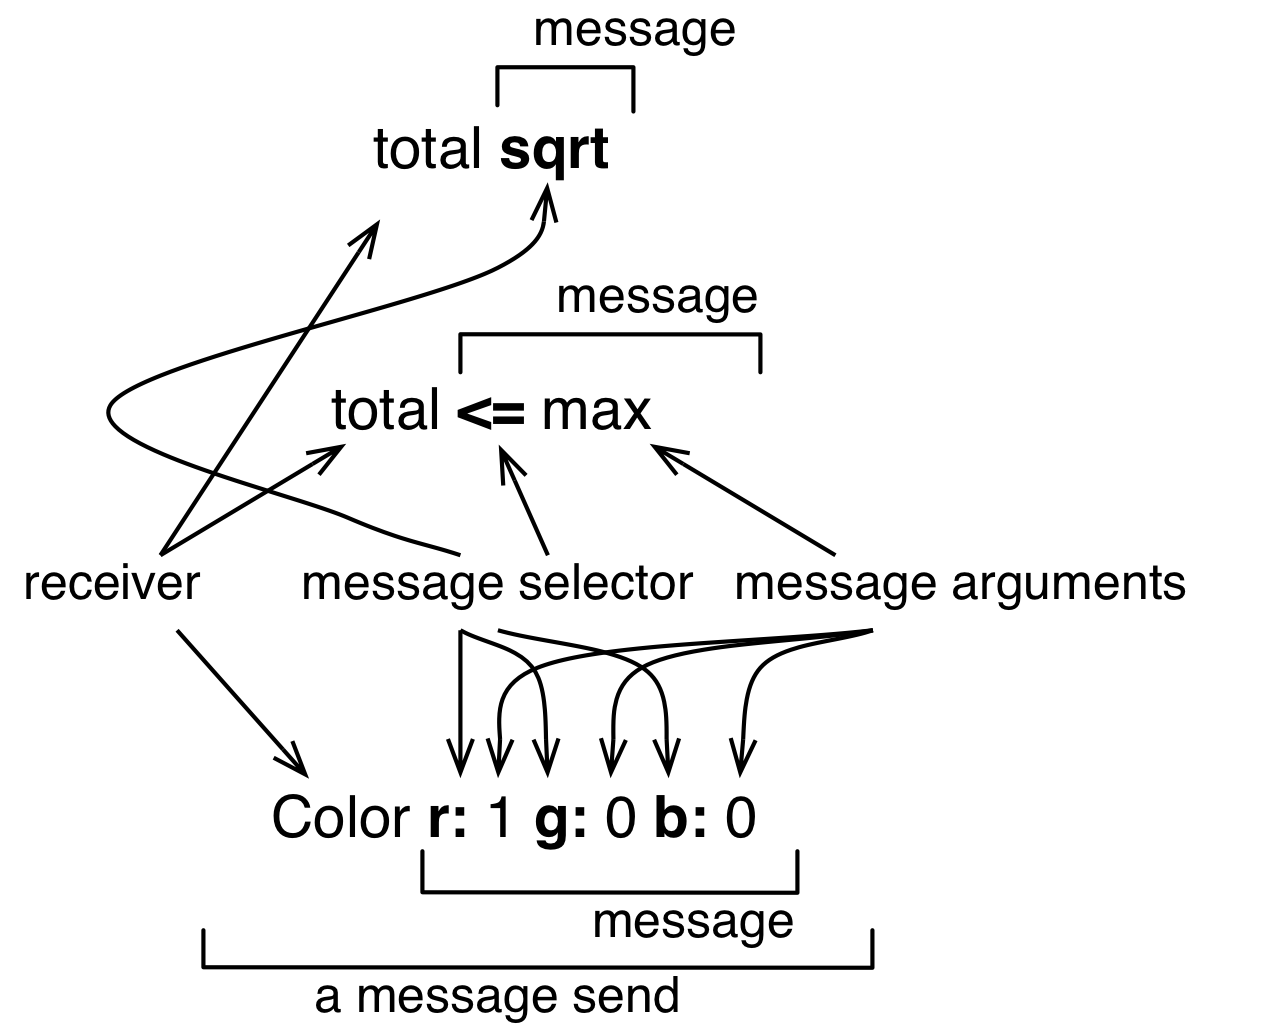
\includegraphics[width=0.7\textwidth]{/Users/ducasse/Workspace/FirstCircle/MyBooks/Bk-Writing/PharoBooks/LearningOOPWithPharoTrans/_result/pdf/Chapters/SyntaxGlimpse/figures/message.png}\caption{Message sends composed of a receiver, a method selector, and a set of arguments.\label{fig:firstScriptMessage}}\end{center}
\end{figure}


A message is always sent to a receiver, which can be a single literal, a block
or a variable or the result of evaluating another message.
\section{Three kind of Messages}
There are three kinds of message: \textit{unary} (without any argument), \textit{binary} (with two arguments) and \textit{keywords} (with arguments).

There are three kinds of messages in Pharo. This distinction has been made to reduce the number of mandatory parentheses.

\begin{enumerate}
\item \textit{Unary} messages take no argument. \textcode{1 factorial} sends the message \textcode{factorial} to the object 1.
\item \textit{Binary} messages take exactly one argument. \textcode{1 + 2} sends the message \textcode{+} with argument 2 to the object 1.
\item \textit{Keyword} messages take an arbitrary number of arguments. \textcode{2 raisedTo: 6 modulo: 10} sends the message consisting of the message selector \textcode{raisedTo:modulo:} and the arguments 6 and 10 to the object 2.
\end{enumerate}
\section{Unary messages}
Unary message selectors consist of alphanumeric characters, and start with a lower case letter.
Here is an example of unary message:

\begin{displaycode}{plain}
20 factorial 
>>> 2432902008176640000
\end{displaycode}

We send the unary message \textcode{factorial} to the number \textcode{20}. Unary means that there is no argument and that the selector is 
composed of letters. 
\section{Binary messages}
Here is an example of binary message:

\begin{displaycode}{plain}
12 + 15 
>>> 27
\end{displaycode}

We send the binary message \textcode{+} to the number \textcode{12} with the argument \textcode{15}. 
A binary message is defined by a binary selector: a selector written without alphabetic characters, i.e., such \textcode{+-/*=\textasciitilde{} \textless{} \textgreater{}}.
Binary message selectors consist of one or more characters from the following set:

\begin{displaycode}{plain}
+ - / \ * ~ < > = @ % | & ? ,
\end{displaycode}
\section{Keyword messages}
Keyword messages are messages with arguments. 
Keyword message selectors consist of a series of alphanumeric keywords, where
each keyword starts with a lower-case letter and ends with a colon.

For example to access the element of an array we send the message \textcode{at:} with as argument the index in the array. Arrays have their first element at index 1. 

\begin{displaycode}{plain}
#(11 22 33) at: 2
>>>22
\end{displaycode}

Another keyword-based message is the message \textcode{at:put:} to change the value of an array. 
Here we put the number 66 in the second position. 

\begin{displaycode}{plain}
| a |
a := #(11 22 33).
a at: 2 put: 66.
a
>>>#(11 66 33)
\end{displaycode}

Another example 

\begin{displaycode}{plain}
1 between: 0 and: 3 
>>> true
\end{displaycode}

This message would expressed in C-like syntax as follows: 

\begin{displaycode}{plain}
1.betweenAnd(0,3) 
>>> true
\end{displaycode}
\section{Execution order and parentheses}
The order in which messages are sent is determined by the type of
message. There are just three types of messages: \textbf{unary}, \textbf{binary}, and \textbf{keyword
messages}. Pharo distinguishes such three types of messages to minimize the number of parentheses. 

\begin{itemize}
\item Unary messages are always sent first, then binary messages and finally keyword ones. 
\item As in most languages, parentheses can be used to change the order of execution.
\end{itemize}

These rules make Pharo code as easy to read as possible. And most of the time you do not have to think about the rules.

\begin{displaycode}{plain}
(4 + 4) * 5
>>> 40
\end{displaycode}

\begin{displaycode}{plain}
2 raisedTo: 1 + 3 factorial
>>> 128
\end{displaycode}

First we send \textcode{factorial} to 3, then we send \textcode{+ 6} to 1, and finally we
send \textcode{raisedTo: 7} to 2. Recall that we use the notation expression \textcode{--\textgreater{}}
to show the result of evaluating an expression.

Precedence aside, execution is strictly from left to right, so:

\begin{displaycode}{plain}
1 + 2 * 3 
>>> 9
\end{displaycode}

return 9 and not 7. Parentheses must be used to alter the order of evaluation:

\begin{displaycode}{plain}
1 + (2 * 3) 
>>> 7
\end{displaycode}
\section{Sending multiple messages to the same object}
Message sends may be composed with periods and semi-colons. A period separated
sequence of expressions causes each expression in the series to be evaluated as
a \textit{statement}, one after the other.

\begin{displaycode}{plain}
Transcript cr.
Transcript show: 'hello world'.
Transcript cr
\end{displaycode}

This will send \textcode{cr} to the \textcode{Transcript} object, then send it \textcode{show: 'hello world'}, and finally send it another \textcode{cr}.

When a series of messages is being sent to the \textit{same} receiver, then this can
be expressed more succinctly as a \textit{cascade}. The receiver is specified just
once, and the sequence of messages is separated by semi-colons:

\begin{displaycode}{plain}
Transcript
  cr;
  show: 'hello world';
  cr
\end{displaycode}

This has precisely the same effect as the previous example.
\section{Blocks}
Blocks (lexical closures) provide a mechanism to defer the execution of expressions. A block is
essentially an anonymous function with a definition context. A block is executed by sending it the
message \textcode{value}. The block answers the value of the last expression in its
body, unless there is an explicit return (with \string^) in which case it returns the value of the returned expression.

\begin{displaycode}{plain}
[ 1 + 2 ] value 
>>> 3
\end{displaycode}

\begin{displaycode}{plain}
[ 3 = 3 ifTrue: [ ^ 33 ]. 44 ] value
>>> 33
\end{displaycode}

Blocks may take parameters, each of which is declared with a leading colon. A
vertical bar separates the parameter declaration(s) from the body of the block.
To evaluate a block with one parameter, you must send it the message value: with
one argument. A two-parameter block must be sent \textcode{value:value:}, and so on, up
to 4 arguments.

\begin{displaycode}{plain}
[ :x | 1 + x ] value: 2 
>>> 3
[ :x :y | x + y ] value: 1 value: 2 
>>> 3
\end{displaycode}

Blocks may also declare local variables, which are surrounded by vertical bars,
just like local variable declarations in a method. Locals are declared after any
arguments:

\begin{displaycode}{plain}
[ :x :y |
	| z |
	z := x + y.
	z ] value: 1 value: 2 
>>> 3
\end{displaycode}

Blocks are actually lexical closures, since they can refer to variables of the
surrounding environment. The following block refers to the variable \textcode{x} of its
enclosing environment:

\begin{displaycode}{plain}
| x |
x := 1.
[ :y | x + y ] value: 2 
>>> 3
\end{displaycode}

Blocks are instances of the class \textcode{BlockClosure}. This means that they are
objects, so they can be assigned to variables and passed as arguments just like
any other object.
\section{Method syntax}
Whereas expressions may be evaluated anywhere in Pharo (for example, in a
playground, in a debugger, or in a browser), methods are defined in a
 class using a code browser, or in the debugger. Methods can also be filed in from an
external medium, but this is not the usual way to program in Pharo.

Programs are developed one method at a time, in the context of a given class. A
class is defined by sending a message to an existing class, asking it to create
a subclass, so there is no special syntax required for defining classes.

Here is the method \textcode{lineCount} in the class \textcode{String}. The usual \textit{convention}
is to refer to methods as \textcode{ClassName\textgreater{}\textgreater{}methodName}. Here the method is then \textcode{String\textgreater{}\textgreater{}lineCount}.
Note that \textcode{ClassName\textgreater{}\textgreater{}} is not part of the Pharo syntax just
a convention used in books to clearly define a method. It means that when you define it you should
 just type the selector (here \textcode{lineCount}). 

\begin{displaycode}{plain}
String >> lineCount
	"Answer the number of lines represented by the receiver, where every cr adds one line."

	| cr count |
	cr := Character cr.
	count := 1 min: self size.
	self do: [:c | c == cr ifTrue: [count := count + 1]].
	^ count
\end{displaycode}

Syntactically, a method consists of:

\begin{enumerate}
\item the method pattern, containing the name (i.e., \textcode{lineCount}) and any arguments (none in this example)
\item comments (these may occur anywhere, but the convention is to put one at the top that explains what the method does)
\item declarations of local variables (i.e., \textcode{cr} and \textcode{count}); and
\item any number of expressions separated by dots (here there are four).
\end{enumerate}

The execution of any expression preceded by a \textcode{\string^} (a caret or upper
arrow, which is Shift-6 for most keyboards) will cause the method to exit at
that point, returning the value of that expression. A method that terminates
without explicitly returning some expression will implicitly return \textcode{self}.

Arguments and local variables should always start with lower case letters. Names
starting with upper-case letters are assumed to be global variables. Class
names, like \textcode{Character}, for example, are simply global variables referring to
the object representing that class.
\section{Some conditionals}
Pharo offers no special syntax for control constructs. Instead, these are
typically expressed by sending messages to booleans, numbers and collections,
with blocks as arguments.

Conditionals are expressed by sending one of the messages \textcode{ifTrue:},
\textcode{ifFalse:} or \textcode{ifTrue:ifFalse:} to the result of a boolean expression. 

\begin{displaycode}{plain}
(17 * 13 > 220)
	ifTrue: [ 'bigger' ]
	ifFalse: [ 'smaller' ] 
>>>'bigger'
\end{displaycode}

Note that the order can be reserved too.

\begin{displaycode}{plain}
(17 * 13 > 220)
	ifFalse: [ 'smaller' ]
	ifTrue: [ 'bigger' ]
>>>'bigger'
\end{displaycode}
\section{Some loops}
Loops are typically expressed by sending messages to blocks, integers or
collections. Since the exit condition for a loop may be repeatedly evaluated, it
should be a block rather than a boolean value. Here is an example of a very
procedural loop:

\begin{displaycode}{plain}
n := 1.
[ n < 1000 ] whileTrue: [ n := n*2 ].
n 
>>> 1024
\end{displaycode}

The message \textcode{whileFalse:} reverses the exit condition.

\begin{displaycode}{plain}
n := 1.
[ n > 1000 ] whileFalse: [ n := n*2 ].
n 
>>> 1024
\end{displaycode}

The message \textcode{timesRepeat:} offers a simple way to implement a fixed iteration:

\begin{displaycode}{plain}
n := 1.
10 timesRepeat: [ n := n*2 ].
n 
>>> 1024
\end{displaycode}

We can also send the message \textcode{to:do:} to a number which then acts as the
initial value of a loop counter. The two arguments are the upper bound, and a
block that takes the current value of the loop counter as its argument:

\begin{displaycode}{plain}
result := String new.
1 to: 10 do: [:n | result := result, n printString, ' '].
result 
>>> '1 2 3 4 5 6 7 8 9 10'
\end{displaycode}
\section{Iterators}
Collections comprise a large number of different classes, many of which support the same set of messages.
The most important messages for iterating over collections include \textcode{do:}, \textcode{collect:}, \textcode{select:},
\textcode{reject:}, \textcode{detect:} and \textcode{inject:into:}. These messages define high-level
iterators that allow one to write very compact code.

An \textbf{Interval} is a collection that lets one iterate over a sequence of numbers
from the starting point to the end. \textcode{1 to: 10} represents the interval from 1
to 10. Since it is a collection, we can send the message \textcode{do:} to it. The argument
is a block that is evaluated for each element of the collection.

\begin{displaycode}{plain}
result := String new.
(1 to: 10) do: [:n | result := result, n printString, ' '].
result 
>>> '1 2 3 4 5 6 7 8 9 10 '
\end{displaycode}

The message \textcode{collect:} builds a new collection of the same size, transforming each
element. (You can think of \textcode{collect:} as the Map in the MapReduce
programming model).

\begin{displaycode}{plain}
(1 to:10) collect: [ :each | each * each ] 
>>> #(1 4 9 16 25 36 49 64 81 100)
\end{displaycode}

The messages \textcode{select:} and \textcode{reject:} build new collections, each containing a subset of
the elements satisfying (or not) the boolean block condition.

The message \textcode{detect:} returns the first element satisfying the condition. Don't forget
that strings are also collections (of characters), so you can iterate over all
the characters.

\begin{displaycode}{plain}
'hello there' select: [ :char | char isVowel ] 
>>> 'eoee'
'hello there' reject: [ :char | char isVowel ] 
>>> 'hll thr'
'hello there' detect: [ :char | char isVowel ] 
>>> $e
\end{displaycode}

More about collections can be found in Pharo by Example.
\section{Chapter summary}
\begin{itemize}
\item Pharo has  some reserved identifiers (also called pseudo-variables): \textcode{true}, \textcode{false}, \textcode{nil}, \textcode{self} and \textcode{super}.
\item There are five kinds of literal objects: numbers (5, 2.5, 1.9e15, 2r111), characters (\textcode{\$a}), strings (\textcode{'hello'}), symbols (\textcode{\#hello}), and arrays (\textcode{\#('hello' \#hi)} or \textcode{\{ 1 . 2 . 1 + 2 \}} )
\item Strings are delimited by single quotes, comments by double quotes. To get a quote inside a string, double it.
\item Unlike strings, symbols are guaranteed to be globally unique.
\item Use \textcode{\#( ... )} to define a literal array. Use \textcode{\{ ... \}} to define a dynamic array.  
\item There are three kinds of messages: unary (e.g., \textcode{1 asString}, \textcode{Array new}), binary (e.g., \textcode{3 + 4}, \textcode{'hi', ' there'}), and keyword (e.g., \textcode{'hi' at: 2 put: \$o})
\item A cascaded message send is a sequence of messages sent to the same target, separated by semi-colons: 
\item Local variables are declared with vertical bars. Use \textcode{:= } for assignment. \textcode{\textbar{}x\textbar{} x := 1 }
\item Expressions consist of message sends, cascades and assignments, evaluated left to right (and optionally grouped with parentheses). Statements are expressions separated by periods.
\item Block closures are expressions enclosed in square brackets. Blocks may take arguments and can contain temporary variables. The expressions in the block are not evaluated until you send the block a value message with the correct number of arguments. \textcode{{[} :x \textbar{} x + 2 {]} value: 4}
\item There is no dedicated syntax for control constructs, just messages that conditionally evaluate blocks.
\end{itemize}


% lulu requires an empty page at the end. That's why I'm using
% \backmatter here.
\backmatter

% Index would go here
\bibliographystyle{abbrv}
\bibliography{others.bib}
\end{document}
